%%
%% This is file `sduthesis-demo.tex',
%% generated with the docstrip utility.
%%
%% The original source files were:
%%
%% sduthesis.dtx  (with options: `demo')
%% 
%% -----------------------------------
%% 
%% This is a generated file.
%% 
%% Copyright (C) 2012 -- 2014 by Liam Huang
%% 
%% This work may be distributed and/or modified under the
%% conditions of the LaTeX Project Public License, either version 1.3
%% of this license or (at your option) any later version.
%% The latest version of this license is in
%%   http://www.latex-project.org/lppl.txt
%% and version 1.3 or later is part of all distributions of LaTeX
%% version 2005/12/01 or later.
%% 
%% This work has the LPPL maintenance status `maintained'.
%% 
%% The Current Maintainer of this work is Liam Huang.
%% 
%%
%% 2019 03 28 Xian-Yu Wang modified this file and made a SDU(wh) test version.
%% If you encounter any problem that you can not solve it by reading sduthesis.pdf, you can report it to me.
%% My e-mail: xianyuwang7@gmail.com

\documentclass[openany]{sduthesis} %%openany 章节从任意页面开始

\StuNum{201400830000}         % 学号
\Ctitle{SDU(wh)本科毕业论文模版\\修改自Liam Huang的模版} % 中文标题
\Cauthor{文心湖}             % 作者中文名
\Dpart{五四广场研究院}               % 学院
\Cmajor{玛珈山车技研究} % 专业中文名
\Grade{9102级}                % 年级
\Csuperver{楼化水~~教授}        %指导老师中文名

\Cdate{\today}
\title{\the\Ctitle}
\author{\the\Cauthor}
\date{\the\Cdate}
\usepackage{tikz}
\usepackage{subfig}
\usepackage{tabu}
\usepackage{booktabs}
\usepackage{hyperref }
\usepackage{pgf} % for the calculation
\begin{document}
\maketitlepagestatement

\begin{cnabstract}

山东大学简称山大,最早可以追溯到 1901 年清朝政府建立的「山东大学堂」,她是中国第二所国立大学,也是第一所具有完整宪章的大学。2001 年,原山东大学、山东医科大学和山东工业大学合并组建成新的山东大学。

离开山大之后,思思念念的是山大的美景、美食和美人。这篇文章简介了山大的历史和现状,并图文并茂地展现了山大校园之美,同时也以实例的方式给出了模板的用法。

\cnkeywords{山东大学,美景,模板}
\end{cnabstract}
\begin{enabstract}
Shandong University, referred to SDU, was set up in the year 1901 in the name of The Advanced School of Shandong (山东大学堂). She is the second national unversity of China, as well as the first unversity that has a complete constitution. In the year 2001, the original Shandong Unversity, Shandong Medical University and Shandong Industry Unversity merge with each other and became the new Shandong University.

Graduting from SDU, I am suffering from lovesickness for the beauties, say the beautiful scenery, the beautiful teachers and the tasty food. This article introduces the history and current status of Shandong Unversity and present the beautiful scenery of Shandong Unversity, and gives a demo to the thesis template at the same time.

\enkeywords{Shandong Unversity, Beautiful scenery, Thesis Template}
\end{enabstract}


\tableofcontents





\chapter{介绍}
山东大学简称山大,是中国著名大学,是教育部直属的综合性全国重点大学。

文章的第二章介绍了山东大学的历史,第三章介绍了山东大学的现状,第四章介绍了山东大学特别是济南中心校区的美景,附录是研究生院对学位论文的格式要求。
\chapter{山东大学的历史}

1901年:山东巡抚袁世凯(清光绪二十七年)上奏《山东试办大学堂暂行章程折稿》,同时调蓬莱知县李于锴进行筹备。是年11月《折稿》获准,在济南泺源书院正式创办了官立山东大学堂。首任 校长是政界闻人唐绍仪(时称管理总办)。第一批招收学生300人,分专斋、正斋、备斋、分斋督课。 聘请中西教习50余人,后增至110多人,美国人赫士为总教习。课程设置除经史子集外,还有社会科学、自然科学和外国语等20多门。学制初为三年,后改为四年。1904年学校迁入济南杆石桥新址,改为山东高等学堂。 1911年又改称山东高等学校。周学熙、方燕年、陈恩焘、萧应椿、陈庆和、周学渊、魏业锐、陈恩 畲、李豫同、李联璧、范之杰、黄国恩、丁维椽等先后出任校长。 1914年国民党政府实行全国设立大学区,各区中心城市设大学,各省设专门学校的体制,山东隶属中心城市北平,按章大学堂停办。师生分别转入法政、工业、农业、商业四个专门学校,校长丁维椽继任商业专门学校校长,校舍由法政专门学校使用。 山东大学堂在建校14年中,共培养毕业生770人,选送去欧美和日本留学的59人。其中徐镜心、 张伯言等人在日本参加同盟会,被孙中山先生委任为山东同盟会负责人。山东大学堂是山东省第一所官办的高等学校,也是山东大学历史的起点。

1906在年济南皇华馆设立法政学堂。翌年再设法律学堂,时称第一、第二法政学堂。1913年合并为山东公立法政专门学校。 1906年,山东巡抚杨士骧、吴廷斌又在济南东关全福庄设立山东高等农业学堂,以南郊千佛山、马鞍山北麓五千亩土地作为学堂的林场,1913年易名山东公立农业专门学校。 1912年,留日学生叶春墀请准在济南南关设立商业学校,随后定名山东公立商业专门学校. 1912年,青州府高密中等工业学堂和济南工业学堂合并,后又并入山东第一中学,于第二年在一 中尚志堂校舍成立山东公立工业专门学校。 1915年,山东省设医学传习所,1916年改名为山东省立医学学校,校址在济南北园白鹤庄, 1920年正式命名山东公立医学专门学校。 1920年,又将矿业传习所扩建为山东公立业专门学校,校址设在济南东关。 上述六个专门学校课程均为现代社会科学和自然科学,教师多为欧美和日本留学生,学制一般为 三年,医学四年,十余年共毕业学生4000余人。 1926年,六所专门学校再行合并,组建成为省立山东大学。在山东大学的发展历史上,这六所专门学校起着承前启后的作用。

1926年,奉系军阀张宗昌督鲁,下令将山东公立六个专门学校合并,在济南建省立山东大学,由山东省教育厅厅长,清末状元王寿彭任校长。设文、法、工、农、医五个学院,计有中国哲学、国文学、 法律、政治经济、商学、机械、机织、应用化学、采矿、农学、林学、蚕学、医学13个系,并有附属 中学。校设评议会,院设教务会,系设教授会。定期研究教学、人事、经费等问题。大学部有教师320 人,其中教授给200人,除专业课外,并开设选修课,学生毕业授学士学位。 1928年,国民北伐军进抵山东,奉系军阀败逃。日本帝国主义借口保护侨民出兵济南,制造了「五、三」惨案。在动乱中,学校经费无着,随即停办。 1924年8月正式创立私立青岛大学,高恩洪自任校长。设工科和商科,学制四年,学生修业期满 考试及格者授予学士学位。学生除本国外还有南洋华侨和朝鲜学生。革命活动家罗荣桓、彭明晶等系该校学生。校董事会聘请学界名流梁启超、蔡元培、张伯苓、黄炎培等人为名誉董事。选用德国人在青岛建造的俾斯麦兵营作校址。 1925年直奉战争再起,直系军阀失败,高恩洪下野,学校濒于倒闭,校董会公推山东省议长宋传典接任校长,勉强维持。 1928年北伐军进抵山东后,奉系败逃,学校经费逐渐断绝停办,学生按大学结业处理。省立山东大学和私立青岛大学是随后创办的国立青岛大学的前身,在山东大学历史上占有重要篇章。

1928年8月,南京国民政府教育部根据山东省教育厅的报告,下令将省立山东大学改为国立山东大学。并由何思源、魏宗晋、陈雪南、赵畸、王近信、彭百川、杨亮功、杨振声、杜光埙、傅斯年、孙学悟等11人组成国立山东大学筹备委员会,着手筹备工作。在筹备过程中,蔡元培先生力主将国立山东大学设在青岛,取得教育部长蒋梦麟的同意。 1928年6月, 国立山东大学筹备委员会奉令改为国立青岛大学筹备委员会,除接收省立山东大 学外,并将私立青岛大学校产收用,筹备国立青岛大学。1930年5月,国民党政府任命杨振声为校长,9月21日,举行开学典礼,国立青岛大学正式成立。学校初设文、 理、教育三个学院,分为中国文学系、外国文学系、数学系、物理系、化学系、生物学系、教育行政系和乡村教育系八个系。1932 年9月,教育学院停办,学生大部分转入国立中央大学教育学院。同时增设工、农两学院。工学院设 土木工程学系和机械工程学系。农学院设于济南,设研究、推广两部。不久,又将文、理两学院合并 为文理学院。学校设校务会议,由校长、教务长、秘书长、各学院院长、各学系主任和教授代表组成,负责议决一切重大事项。校长杨振声思想进步,富有远见,效法北京大学「兼容并包」、「科学民主」 的办学方针,广聘专家学者,如闻一多、黄敬思、黄际遇、任之恭、傅鹰、沈从文、梁实秋、闻在宥、 游国恩、曾省、汤腾汉等著名学者均在校任教。学校发展较快,声誉日隆,国立青岛大学由此崭露头角。 1931年行政院议决,将国立青岛大学改为国立山东大学,任命赵太侔(赵畸)接任校长。赵太侔 原为国立青岛大学教务长,赞同杨振声的办学方针。接任后增聘老舍、洪深、张煦、丁山、王淦昌、童第周、曾呈奎等一批专家学者,师资阵营更为整齐,同时撙节行政费用,添购图书、仪器,先后建成科 学馆、工学馆、体育馆、化学馆、水力实验室及实习工厂等,改善了办学条件。此时期由于外部环境 相对稳定,校内人才荟萃,名流云集,师生勤奋教学、成就蜚然,成为学界仰重的国内知名高等学府。 国立山东大学实行「学年学分制」,学制四年,学生毕业授学士学位。学校先后创办有学术刊物《科 学丛刊》、《文史丛刊》、《励学》、《刁斗》等。 1937年,「七、七」事变,抗日战争爆发。11月国立山东大学由青岛迁往安徽安庆,不久再迁四川万县。图书、仪器、案卷分批运出,损失严重。 1938 年春学校在万县复课,不久教育部下令「暂行停办」。师生分别转入国立中央大学,图书、 仪器、机械分别暂交国立中央图书馆、国立中央大学、国立中央工业职业学校保管使用。 1946年春,经国民政府教育部批准。国立山东大学在青岛复校,赵太侔再任校长。复校后设文、 理、工、农、医五个学院,计有中国文学、历史学、外国文学、数学、物理学、化学、动物学、植物学、 地质矿物学、土木工程学、机械工程学、电机工程学、农艺学、园艺学、水产水15个系,医学院不会 系,并附设一个大学先修班和高级护士学校。各学院学生修业年限为四年,其中工学院五年,医学院 六年,实行分学制和必修制、选修制。1946年10月25日举行开学典型。知名学者王统照、陆侃如、 冯沅君、黄孝纾、丁山、赵纪彬、杨向奎、萧涤非、丁西林、杨肇 、童第周、曾呈奎、王普、郭贻诚、 王恒守、李先正、刘遵宪、朱树屏、严效复、杨宗翰、郑成坤、李士伟、沈福彭等应聘来校执教。 1949年6月2日青岛解放、王哲、罗竹风、高剑秋率领军管小组进校,对学校进行接管整顿,山 东大学从此进入新的时期。

1945年中共华中局决定,在华中党校基础上,创办华中建设大学。校址设于苏皖边区的旰眙县新埔由华中局宣传部长彭康兼任校长。设民政、财政、文艺三系和一个高干班。首届招生。同年5月4日,正式开学。8月份,首届学生结业,学校迁清江市。1946年初,校长彭康率领部分干部教师和学员北上并入临沂山东大学,华中建设大学校长由李亚农继任,解放区知名人士贺希明、张劲夫、张茜、夏征农、戴白韬、阿英、孙冶芳、范长江、车载、朱维基、黎冰鸿、黄源、陶官云等在校工作和执教。学校拟办成一所正规大学,设工、农、文、医、师范、社会科学等六个学院和预科。 1945年8月,山东抗日人民政府在解放区临沂, 创办了山东大学(为了区别国立山东大学)称临沂 山东大学),由李澄之、田佩之任正副校长。设预科部,招收知识青年,进行思想政治教育。 1946年初,华中建设大学校长彭康,率领该校师生400余人北上,并入临沂山东大学。师资力量 得到充实,学校规模有所扩大,设立政治、经济、教育、文艺四系,转入以专业为主的学习,解放区 教育界的知名人士何封、薛暮桥、李仲融、王淑明、孙克定、刘力行、胡考、宋日昌、尚钺、宋之的等在校执教。 1948年夏,中共华东局决定,以原临沂山东大学渤海地区的部分留守人员为基础,并集中原来的 一些教师,会同华中建设大学的部分干部教师,在潍县组建成立华东大学,同年9月4日开学。韦悫 任校长,张勃川、李宇超任副校长。济南解放后,于11月迁入济南。迁济后成立文学、社会科学、教 育三个学院和一个研究部。另设附属中学。 1949年5月, 韦悫调任上海市副市长,彭康接任校长,学校向正规化大学过渡。11月,教育学 院划出,后成为山东师范学院。附属中学交济南市领导,改为实验中学。1950年全国教育工作会议 后,学校调整为政治、文学、史地、艺术、俄文五系,转入正规化的业务学习。1950年冬奉命迁青 岛,1951年在青岛与山东大学合校。 华中建设大学、临沂山东大学和华东大学,都是短期训练班式的政治大学,在战火纷飞的年代, 为国家培养了近一万名干部,为革命战争和建设作出了积极的贡献。

1951年3月, 山东大学和华东大学合校,仍名 为山东大学。华岗任校长兼校党委书记,童第周、陆侃如为副校长、设文、理、工、农、医五个学院,分中国文学、历史学、外国文学、数学、物理学、化学、动物学、植物学、地质矿物学、水产学、土木工程学、机械工程学、电机工程学、农艺学、园艺学、病虫害学、政治 学、艺术学18个系。其中政治和艺术为两个直属系。学校积极贯彻党的教育方针,推进教学改革,大力开展科学研究。1951年创办《文史哲》杂志和《山东大学学报》,开辟了科学园地,促进了学术争鸣。从此山东大学又进入了学术繁荣的新阶段。 1952年夏,进行全国高等院校调整。山东大学根据中央教委部关于高等学校院系调整的方案,调 整出去的院系有: (一)政治系,迁至济南,组成山东政治学校,现为中共山东省委党校。 (二)艺术系戏剧组,迁至上海,与上海戏剧专科学校合并,组建成中央戏剧学院华东分院,现 为上海戏剧学院。 (三)艺术系音乐、美术两组,迁至无锡,与上海美术专科学校、苏州美术专科学校合并,组建 成华东艺术专科学校,现为南京艺术学院。 (四)工学院和土木系,和原山东工学院的土木、纺织系合并,组建成青岛工学院,后又迁至武 汉与有关系科合并,成立武江测绘学院,现为武汉测绘科学大学。 (五)工学院的机械、电机两系,迁至济南,与原山东大学合并,组建成新的山东工学院,现为 山东工业大学。 (六)农学院的农艺、园艺、植物病虫害学三系,迁至济南,与原山东农学院合并,组建成新的 山东农学院,现为山东农业大学。 (七)医学院1956年独立,扩建为青岛医学院。 (八)理学院的地矿系迁至长春,与有关院校系科合并,组建成长春地质学院。 (九)1954年教育部拟改变高等学校的布局,指令由山东大学负责,在郑州筹建一所新的大学, 由山东大学支援师资,即现今的郑州大学。 (十)在迁校济南时,留在青岛的系科,独立建院后,发展成为现在的青岛海洋大学。 山东大学在院系调整中,分出的系科和其他院校组建了十所高等院校,取消了院一级组织,留有 中文、历史、外文、数学、物理、化学、生物、水产八个系,增设海洋学系,建立文学历史和海洋物 理两个研究所,成为教育部直属的以文、理为主的综合大学。中文、历史两专业开始招收研究生,还接收朝鲜、越南、苏联等国的留学生,学校的影响扩及国外。 1955年华岗受诬陷去职,稍后童第周调中国科学院工作。1956年7月山东省副省长晁哲甫出任校长兼 党委书记。1957年外文系师生进入上海外国语学院,外文系撤销。 1958年夏晁哲甫奉调回省,国务院任命成仿吾为校长兼校党委书记。 1958年7月,山东大学归由山东省领导,同年10月奉命迁校济南。文科的中文、历史两系和理科 数学、物理、化学、生物四系搬迁济南,海洋、水产和正筹建的地矿三系留在青岛(后独立为山东海 洋学院)。 这期间根据科学发展和国家建设事业的需要。于1959年秋恢复了外文系,1960年重设政治系, 建成原子能系和电子系,学校由迁济时的6个系10个专业, 增至政治、中文、历史、外文、数学、物 理、化学、生物学、原子能(后学生并入复旦大学,该系撤销)、电子10个系。建立了中国古典文学、 中国现代文学、美国文学、中国古代史、微分方程(控制论)、磁学、晶体、微生物九个校属研究室。 有八个专业接受培养研究生。设有三个专业业余大学,六个专业函授班,并招收函授研究生,在校业余和函授生达到4000人。同时,恢复了外国留学生培养工作。 学校迁济后,从1959年开始兴建新校舍,到1966年「文革」前七年,共建成文史、化学两栋 教学校,6栋学生宿舍楼,三个食堂,13 栋教工宿舍楼和部分辅助用房,总面积五万平方米。全校 九个系分住两地,校部机关和外文、物理、电子、生物四系仍住原处,称老校;政治、中文、历史、 数学、化学五系迁新校舍,称新校。 1961年学校复归中央教育部领导,学校在文史见长的优势中,向社会科学领域开拓;在理科的扬 长避短中,突出数学、磁学、晶体、微生物的六十年代新特色,为学校以后的发展打下了良好的基础。 1966年开始了「文化大革命」。6月殃及山东大学校园, 全校机构随之瘫痪。1967年后,校内山东 头林立,学校的一派组织夺权后,把校名改为「鲁迅大学」,直到1970年才又恢复了山东大学校名。 1970年夏,山东省革命委员会将山东大学一分为三:政治、中文、外文、历史四系南迁曲阜,与曲 阜师范学院合并,改称为山东大学;生物学系迁奉泰安,并入山东农学院;校部机关和数学、物理、 电子、化学、光学(新建)五系留在济南,成立山东科学技术大学。 1973年周恩来总理在病中得悉这一情况,立即签署恢复山东大学原建制的指示,1974年初山东大学 恢复原建制,山东科学技术大学即行撤销。1971年高等学校恢复招生,实行「群众推荐,领导批准, 学校审定」的招生办法,开始招收工农兵学生入学。到1976年共招收五届工农兵学生(学制二、三年), 总计毕业3267人。

1978年由吴富恒出任校长,孙汉卿任校党委书记。 1984年调整领导班子,校长吴富恒退居二线,邓从豪出任校长,戈平主持校党委的工作。这时期,经原教育部批准。 1984年在风景秀丽的海滨城市威海,设立山东大学威海分校。 1987年,校长邓从豪退居二线,由潘承洞任校长。1986年徐豫龙出任校党委书记。1988年,陈之安任党委书记。1996年,曾繁仁教授出任校党委书记。 经过十几年的不懈努力,学校各项事业有长足发展,在学科建设方面,在注重基础学科建设的同时,大力发展了新兴学科、应用学科,由1978年24个专业,发展到1997年14个学院,45个系(教 学部)。有56个本科专业,57个硕士点,17个博士点和3个博士后流动站。有2个国家重点学科,17个山东省重点学科。有2个国家重点实验室,6个山东省重点实验室,一个国家教委部门开放实验 室。1个国家科委技术推广中心,3个山东省技术工程研究中心。 山东大学设有出版社,建成了综合档案馆和博物馆,设立了附属中小学和校医院。有教职工4500 人,校园占地面积3000多亩,建筑面积50万平方米,学校图书馆藏书220万册,出版有《文史哲》、 《山东大学学报》等八种刊物。

1997年,进入「211工程」建设序列。

2000年7月,由原山东大学、原山东医科大学、原山东工业大学合并组建新的山东大学。

2001年2月,进入「985工程」序列。

\chapter{现状}

\section{三城八校}

当前,山东大学在济南、威海和青岛三市共有八个校区。分别是:

\begin{itemize}
  \item 中心校区;
  \item 洪家楼校区;
  \item 趵突泉校区;
  \item 千佛山校区;
  \item 兴隆山校区;
  \item 齐鲁软件园;
  \item 威海校区(威海);
  \item 青岛校区(青岛)。
\end{itemize}

\subsection{中心校区}

中心校区设有以下院系。
\begin{figure}[!htb]
\centering
\includegraphics[width = 0.8\linewidth]{sduthesis-zhixinlou}
\caption{知新楼上的袅袅轻云}\label{fig:zhixinlou}
\end{figure}
\begin{itemize}
  \item 文学与新闻传播学院;
  \item 历史文化学院;
  \item 数学与系统科学学院;
  \item 物理学院;
  \item 化学与化工学院;
  \item 经济学院;
  \item 生命科学学院;
  \item 经济研究院(中心);
  \item 信息科学与工程学院;
  \item 环境科学与工程学院;
  \item 哲学与社会发展学院;
  \item 晶体材料研究所;
  \item 管理学院;
  \item 环境研究院;
  \item 马克思主义学院;
  \item 大学外语教学部;
  \item 国际教育学院;
  \item 文史哲研究院。
\end{itemize}

\subsection{洪家楼校区}

洪家楼校区设有以下院系。

\begin{itemize}
  \item 政治学与公共管理学院;
  \item 法学院;
  \item 艺术学院;
  \item 外国语学院。
\end{itemize}

\subsection{趵突泉校区}

趵突泉校区设有以下院系。

\begin{itemize}
  \item 医学院;
  \item 公共卫生学院;
  \item 口腔医学院;
  \item 护理学院;
  \item 药学院。
\end{itemize}

\subsection{千佛山校区}

千佛山校区设有以下院系。

\begin{itemize}
  \item 材料科学与工程学院;
  \item 机械工程学院;
  \item 控制科学与工程学院;
  \item 能源与动力工程学院;
  \item 电气工程学院;
  \item 土建与水利学院;
  \item 体育学院。
\end{itemize}

\subsection{兴隆山校区}

兴隆山校区设有以下院系。

\begin{itemize}
  \item 材料科学与工程学院;
  \item 机械工程学院;
  \item 控制科学与工程学院;
  \item 能源与动力工程学院;
  \item 电气工程学院;
  \item 土建与水利学院。
\end{itemize}

\subsection{齐鲁软件园}

齐鲁软件园设有以下院系。

\begin{itemize}
  \item 软件学院;
  \item 计算机科学与技术学院;
  \item 加拿大高等教育基础部(2011届·药学院、公共卫生学院、护理学院等)。
\end{itemize}

\subsection{威海校区}

威海校区设有以下院系。

\begin{itemize}
  \item 东北亚学院;
  \item 商学院;
  \item 法学院;
  \item 新闻传播学院;
  \item 翻译学院;
  \item 艺术学院;
  \item 海洋学院;
  \item 机电与信息工程学院;
  \item 空间科学与物理学院;
  \item 继续教育学院;
  \item 数学与统计学院;
  \item 继续教育学院。
\end{itemize}

\subsection{青岛校区}

已建成。

\section{师资力量}

截止2013年,学校有教授1107人,博士生导师907人。其中,诺贝尔物理学奖获得者Peter Grünberg教授加盟山东大学,受聘为特聘教授;山东大学研究生导师莫言教授荣获2012年诺贝尔文学奖。同时,学校有中国科学院和工程院院士9人,双聘院士43人,山东大学终身教授11人,山东大学人文社科一级教授14人;「千人计划」国家特聘教授22人,「青年千人计划」5人;国务院学位委员会学科评议组成员7人;国家百千万人才工程入选者26人;教育部「长江学者奖励计划」特聘教授、讲座教授39人,国家级教学团队8个,长江学者创新团队7个,国家杰出青年基金获得者32人,山东省泰山学者特聘专家教授45位、泰山学者海外特聘专家22位、泰山学者攀登计划人选4位,国家级教学名师9人。

\subsection{两院院士}

\subsubsection{科学院院士}彭实戈、钱逸泰、佟振合。

\subsubsection{工程院院士}艾兴、张运、王文兴、方家熊、钱七虎、张明高。

\section{愉快的吐槽}

关于山东大学的吐槽,见表 \ref{tab:debunk}。

\begin{table}[!htb]
\centering
\caption{学子的吐槽}\label{tab:debunk}
\begin{tabular}{*5{c}}
  \toprule
  & 中心校区 & 洪家楼校区 & 趵突泉校区 & 千佛山校区 \\
  \midrule
  饮食 & 超赞 & 赞 & 赞 & 一般 \\
  住宿 & 比较差 & 很差 & 未知 & 未知\\
  \midrule[0.8pt]
  & 兴隆山校区 & 软件园 & 威海校区 & 青岛校区 \\
  \midrule
  饮食 & 比较差 & 未知 & 赞 & 赞 \\
  住宿 & 未知 & 未知 & 赞 & 赞\\
  \bottomrule
\end{tabular}
\end{table}
\clearpage
\section{功能测试区域}
1. 公式测试:$t_{\mathrm{occ}}(E)=t_{0}+\frac{P_{\mathrm{a}}}{2}+P_{\mathrm{s}} E+\frac{e P_{\mathrm{a}}}{\pi} \cos \omega$  

2. \LaTeX 文献引用环境thebibliography测试\upcite{liu}

3. Bibtex引用文献管理环境测试\cite{DBLP:journals/sac/Braak06}。
Bibtex使用方法:在.bib文件中载入标准文献格式,cite引用,先xelatex,再bibtex,再xelatex

4. 脚注测试\footnote[1]{\label{footnoot1}脚注测试}, 注意,本latex 模板由Ctex中的book类制作。在 article 类型的文件中,脚注是被从头到尾顺序编号的;在 book 和 report 类型文件中,脚注是每一章各自顺序编号的。如果希望脚注是每一章各自顺序编号的,可不添加[]中的数字,否则需要自己编号。BTW,有函数footnpag,但是不好使。


5. Tikz绘图测试,Tikz入门教程:\url{http://www.fuzihao.org/blog/2015/08/11/TikZ%E5%85%A5%E9%97%A8%E6%95%99%E7%A8%8B/}

TikZ and PGF examples:\href{http://www.texample.net/tikz/examples/}{http://www.texample.net/tikz/examples/}


\begin{center}
 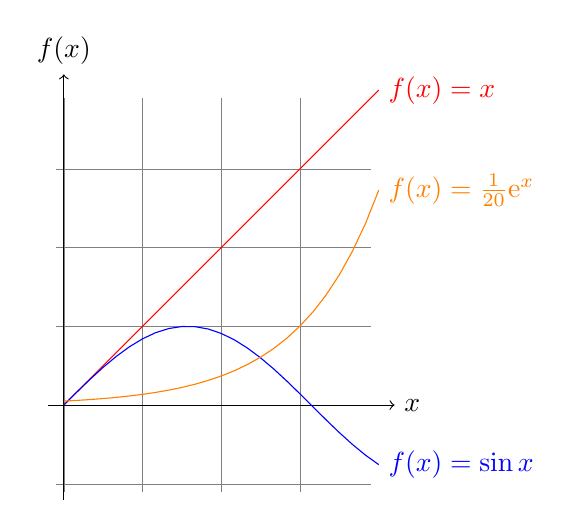
\begin{tikzpicture}[domain=0:4]
  \draw[very thin,color=gray] (-0.1,-1.1) grid (3.9,3.9);
  \draw[->] (-0.2,0) -- (4.2,0) node[right] {$x$};
  \draw[->] (0,-1.2) -- (0,4.2) node[above] {$f(x)$};
  \draw[color=red]    plot (\x,\x)             node[right] {$f(x) =x$};
  % \x r 表示弧度
  \draw[color=blue]   plot (\x,{sin(\x r)})    node[right] {$f(x) = \sin x$};
  \draw[color=orange] plot (\x,{0.05*exp(\x)}) node[right] {$f(x) = \frac{1}{20} \mathrm e^x$};
\end{tikzpicture}
\end{center}



\chapter{山东大学图志:秋忆——山大之恋}

匆匆间,已是初冬。虽置身于这份清冷,我们却还记得独属于秋天的温暖气息。曾经秋风瑟瑟,吹散了大成广场孩童戏水的欢声,也曾暮雨潇潇,滴落了小树林鸟雀低鸣的婉转。山大视点推出“秋忆”系列图志,用相机记录秋日的苒苒物华,探索校园的清秋况味,呈现不一样的秋意山大。

云淡天高雁南渡,空灵明澈掩喧嚣。秋日的山大校园,落叶浸染着大地的金黄,秋林掩映着落日的余红。现在,跟随我们的镜头,一起走进图志:秋忆——山大之恋。

山大的秋天,是……

如图 \ref{fig:zhixinlou}、\ref{fig:xianzhidadao}、\ref{fig:hongloujiaotang}、\ref{fig:weihai}。

\begin{figure}[!htb]
\centering
\includegraphics[width = 0.8\linewidth]{figures/sduthesis-zhixinlou}
\caption{知新楼上的袅袅轻云}\label{fig:zhixinlou}
\end{figure}

\begin{figure}[!htb]
\centering
\subfloat[先志大道的萧萧落叶]{\includegraphics
  [width = 0.45\linewidth]{figures/sduthesis-xianzhidadao}\label{fig:xianzhidadao}}\quad
\subfloat[洪楼教堂的呢喃钟鸣]{\includegraphics
  [width = 0.45\linewidth]{figures/sduthesis-hongloujiaotang}\label{fig:hongloujiaotang}}\quad
\caption{千佛山与洪家楼}
\end{figure}

\begin{figure}[!htb]
\centering
\begin{minipage}{0.5\linewidth}
\centering
\includegraphics[width = 0.95\linewidth]{figures/sduthesis-baotuquan}
\caption{古老号院的安然静谧}\label{fig:baotuquan}
\end{minipage}%
\begin{minipage}{0.5\linewidth}
\centering
\includegraphics[width = 0.95\linewidth]{figures/sduthesis-ruanjianyuan}
\caption{软件园区的日新月异}\label{fig:ruanjianyuan}



\end{minipage}
\end{figure}

\begin{figure}[!htb]
\begin{minipage}{0.5\linewidth}
\centering
\includegraphics[width = 0.95\linewidth]{figures/sduwh.png}
\caption{威海校区的图书馆}\label{fig:weihai}
\end{minipage}
\end{figure}

\begin{thebibliography}{1}
\addcontentsline{toc}{chapter}{参考文献}
\bibitem{liu} 刘海洋. \LaTeX 入门 [M]. 北京: 电子工业出版社, 2013.
\bibitem{hu}  胡伟. \LaTeX 2e完全学习手册(第二版). 北京: 清华大学出版社, 2013.
\end{thebibliography}

 \bibliographystyle{plain} 
\bibliography{reference}
 \addcontentsline{toc}{chapter}{参考文献Bibtex}
 
\chapter*{\zihao{3}注{\quad}{\quad}{\quad}释}
\addcontentsline{toc}{chapter}{注释}
\ref{footnoot1}.脚注测试

\chapter*{\zihao{3} 附{\quad}{\quad}{\quad}录}
\addcontentsline{toc}{chapter}{附录}

\section{山东大学研究生院关于学位论文的格式要求}
因为没有找到关于学士学位论文的格式要求,这里附上一段研究生院的要求,仅供参考。
\subsection{学位论文的基本要求}
硕士学位论文一般应用中文撰写,提倡并鼓励用中、外文撰写。理学、工学、医学类博士学位论文须用中、外文撰写,人文社科类博士学位论文提倡并鼓励用中、外撰写。博士学位论文字数一般3--10万字,摘要为3000字以上;硕士学位论文字数一般2--5万字,摘要为1000字左右。
\subsection{学位论文的结构要求}
博士、硕士学位论文一般应由以下几部分组成,依次为:
\begin{enumerate}
\item 论文封面;\item 扉页;\item 原创性声明和关于论文使用授权的声明;\item 中、外文论文目录;\item 中文摘要;\item 外文摘要;\item 符号说明;\item 论文正文(包括文献综述);\item 附录、附图表;\item 引文出处及参考文献;\item 致谢;\item 攻读学位期间发表的学术论文目录;\item 学位论文评阅及答辩情况;\item 外文论文。
\end{enumerate}
\subsection{学位论文的格式要求}
\subsubsection{论文封面}
采用研究生院统一印制的封面。封面的论文题目需要中、外文标示。用小二号加重黑体字打印封面的中文论文题目,用三号加重打印封面外文论文题目,四号加重黑体字打印脊背处论文题目和封面作者姓名、专业、指导教师、合作导师姓名和专业技术职务、论文完成时间、密级、学校代码、学号、分类号等内容。论文题目不得超过30个汉字。分类号须采用《中国图书资料分类法》进行标注。
\subsubsection{扉页}
论文设扉页,其内容与封面相同,送交校学位办公室、图书馆和档案馆的论文其扉页由本人用碳素钢笔填写。
\subsubsection{原创性声明和关于学位论文使用授权的说明}
论文作者和指导教师在向校学位办公室、图书馆、档案馆提交论文时必须在要求签名处签字。
\subsubsection{论文目录}
论文需要有中外文目录各一份。目录应将文内的章、节标题依次排列,并注明页码。标题应简明扼要。中文的「目录」标题字用小三号加重黑体字打印,目录内容用小四号宋体打印。外文的「目录」标题字用加重小三号字体大写字母打印,目录内容用小四号字体小写字母打印。
\subsubsection{中文摘要}
中文摘要应以最简洁的语言介绍论文的内容要点,其中包括研究目的、研究方法、结果、结论及意义等,并注意突出论文中的新论点、新见解或创造性的成果,并在摘要后列出3--5个关键词,之间用分号相隔。关键词应体现论文的主要内容,词组符合学术规范。「中文摘要」 标题字用小三号加重黑体字打印,摘要内容用小四号宋体打印。
\subsubsection{外文摘要}
外文摘要内容应与中文摘要基本一致,要语句通顺,语法正确,准确反映论文的内容,并在其后列出与中文相对应的外文关键词。「摘要」标题字用加重小三号字体大写字母打印,摘要内容用小四号字体小写字母打印。
\subsection{符号说明}
介绍论文中所用符号表示的意义。
\subsubsection{论文正文}
正文是学位论文的主体和核心部分。论文应在前言中包含必要的文献综述,并用小标题标明。论文中的计量单位、制图、制表、公式、缩略词和符号必须遵循国家规定的标准。其行文方式和文体的格局,研究生可根据自己研究课题的表达需要不同而变化,灵活掌握。论文题目用小三号黑体字打印,内容用小四号宋体打印,一般每行32--34字,每页29--31行。每页要有页眉,其上居中打印「山东大学博(硕)士学位论文」字样,页码标注在页面低端(页角)外侧。 论文中的章的标题用小三号加重黑体;节的标题用四号加重黑体;目及子目以下的标题用小四号加重黑体打印,标题应简明扼要,体现阐述内容的重点,无标点符号。
\subsubsection{附录、附图表}
主要列入正文内过分冗长的公式推导,供查读方便所需的辅助性数学工具或表格;重复性数据图表;实验性图片;程序全文及说明等。
\subsubsection{引文出处及参考文献}
人文社科类学位论文应有详细的引文出处,格式应规范,一般标注于论文每一页的下方或每一章节的结尾位置。参考文献按文中使用的顺序列出,并注明文献的作者、题名、刊物(出版社)名称、出版时间、页码等。理学、工学、医学类学位论文按国际惯例执行。
\subsubsection{致谢}
系对给予各类资助、指导和协助完成研究工作以及提供各种对论文工作有利条件的单位和个人表示的感谢。致谢应实事求是,切忌浮夸之词。
\subsubsection{攻读学位期间发表的学术论文目录}
按学术论文发表的时间顺序,列出本人在攻读学位期间发表或已录用的主要学术论文清单,包括顺序号、论文题名、刊物名称、卷册号及年月、起止页码、论文署名位次。
\subsubsection{学位论文评阅及答辩情况}
论文答辩通过后,送校学位办公室、图书馆和档案馆的论文需将学位论文评阅及答辩情况填入《学位论文评阅及答辩情况表》中。
\subsubsection{外文论文}
\subsubsection{外文论文写作的形式}
可根据本学科的实际选择以下写作形式的其中一种。
\begin{enumerate}
\item 与中文全文在内容和形式上完全一致的外文全文;
\item 两篇以上与学位论文相关的可以在外文期刊上发表(含已发表)的外文论文。
\end{enumerate}
\subsubsection{外语写作的要求}
学位论文外语写作要语句通顺,语法正确,符合该种语言的写作规范,能准确反映作者的学术思想。论文内容用小四号字体小写字母打印。
\subsection{学位论文的打印与装订}
论文用A4标准纸输出,双面打印。博士学位论文一式25份,硕士学位论文一式15份,装订成册,并按要求送交有关部门(送校图书馆和档案馆的论文需线装)。中、外文学位论文原则上一起装订,如篇幅过长可分别装订。除外语专业的学位论文外,其它学科的学位论文一律中文论文在前,外文论文在后。
\vfill
\hfill\begin{minipage}{.3\textwidth}
山东大学研究生院
二〇〇六年十一月十日
\end{minipage}
\section{山东大学威海研究生院关于学位论文的格式要求}
%%\addcontentsline{toc}{section}{B.山东大学威海研究生院关于学位论文的格式要求}
\subsection{目录}
目录:另起页;标题使用3号黑体字,“目录”两字中间空3个汉字字符格;内容使用4号宋体字,要求标明页码,每项内容与对应的页码之间要求使用省略号分隔开。
\subsection{中文摘要}
中文摘要(含关键词):另起页;标题使用3号黑体字,两个标题各自独占行,居中,“摘要”两字中间空3个汉字字符格,“关键词”三字每两字中间空1个汉字字符格;内容使用4号宋体字,单倍行距。
\subsection{英文摘要}
英文摘要(含关键词):与中文摘要和关键词同页;标题使用小2号Times New Roman字体,两个标题各自独占行,居中;内容使用小3号Times New Roman字体,单倍行距。
\subsection{正文}
正文 :另起页;
正文文中标题:
\subsubsection{一级标题}
    一级标题:标题序号为“一、”, 4号黑体字,独占行,末尾不加标点符号。
\subsubsection{二级标题}
  二级标题:标题序号为“(一)”与正文字号相同,独占行,末尾不加标点符号。
  \subsubsection{三级标题}
 三级标题:标题序号为“ 1. ”与正文字号、字体相同。
 \subsubsection{四级标题}
    四级标题:标题序号为“(1)”与正文字号、字体相同。
 \subsubsection{五级标题}
五级标题:标题序号为$\circled{1}$与正文字号、字体相同。
其它内容全部使用小4号宋体字,单倍行距。
\paragraph{五级标题测试}~{}
\newline
五级标题测试

\subsection{参考文献}
参考文献:另起页;标题使用3号黑体字,标题汉字之间无空格,独占行,居中;内容使用小4号宋体字,单倍行距。
\subsection{注释}
注释:另起页;标题使用3号黑体字,“注释”两字中间空3个汉字字符格,独占行,居中;内容使用小4号宋体字,单倍行距。
\subsection{附录}
附录:另起页;标题使用3号黑体字,“附录”两字中间空3个汉字字符格,独占行,居中;内容使用小4号宋体字,单倍行距。
\subsection{谢辞}
谢辞:另起页;标题使用3号黑体字,“谢辞”两字中间空3个汉字字符格,独占行,居中;内容使用4号宋体字,单倍行距。
\subsection{封底}
封底:另起页,空白。


\clearpage
\chapter*{\zihao{3} 谢{\quad}{\quad}{\quad}辞}
\addcontentsline{toc}{chapter}{谢辞}
\zihao{4}
\center

学无止境,气有浩然。

凡我在处,便是山大。
\clearpage
\end{document}
%% 
%% Copyright (C) 2012 -- 2014 by Liam Huang
%% 
%% This work may be distributed and/or modified under the
%% conditions of the LaTeX Project Public License, either version 1.3
%% of this license or (at your option) any later version.
%% The latest version of this license is in
%%   http://www.latex-project.org/lppl.txt
%% and version 1.3 or later is part of all distributions of LaTeX
%% version 2005/12/01 or later.
%% 
%% This work has the LPPL maintenance status `maintained'.
%% 
%% The Current Maintainer of this work is Liam Huang.
%% 
%% -----------------------------------
%% 
%% This work consists of the file  sduthesis.dtx and sduthesis.ins
%% and the derived files           sduthesis.cls,
%%                                 sduthesis-cover.def,
%%                                 sduthesis-statement.def,
%%                                 figures/,
%%                                 sduthesis-demo.tex,
%%                                 README.md,
%%                                 LICENSE.md,
%%                                 sduthesis.pdf and
%%                                 sduthesis-demo.pdf.
%%
%% End of file `sduthesis-demo.tex'.